\section{Technical Proofs}
\label{sec:proofs}

\subsection{Proof of Lemma~\ref{lem:indep}}
\label{proof:lem:indep}

%\begin{pot}
  To analyze the decrease of the potential function, we distinguish
  different cases that corresponds to processors that are executing
  work, sending or answering work requests.  We show that each case
  contributes to a diminution of the potential.

  Between time $k\lambda$ and $(k+1)\lambda$, a processor does (at
  least) one the following four things.  These cases cover all
  possible behaviors of the processor.
  % \begin{enumerate}
  % \item The processor is executing and sending work.
  % \item The processor is executing work and available to respond to the work requests sent by idle processors.
  % \item The processor is executing work and will be idle soon.
  % \item The processor is idle.
  % \end{enumerate}
  % We analyse below how much each case contributes to the decrease of
  % the potential.
  \begin{cases}
  \item ($s_i>0$) The processor started to send work to another (idle)
    processor $j$ before time $k\lambda$.  This means that 
    processor $j$ will receive $s_i(k)$ tasks at a time
    $t<(k+1)\lambda$. Note that by assumption, $s_i(k)\ge w_i(k)$
    because processor $i$ has executed some if its own work since
    it started to send half of its work to $j$.  There are two 
    subcases:
    \begin{itemize}
    \item \textbf{Case~1a}. If no additional work requests have been
      received between $t$ and $(k+1)\lambda$, it holds that
      \begin{align*}
        &w_i(k+1)\le w_i(k)\\
        &w_j(k+1)\le s_i(k)\\
        &s_i(k+1)=s_j(k+1)=0. 
      \end{align*}
      This implies that the potential of $i$ and $j$ at time step
      $k+1$ satisfies:
      \begin{align*}
        \phi_i(k+1)+\phi_j(k+1)
        &= w_i(k+1)^2 + w_j(k+1)^2 + 2(s_i(k+1)^2+s_j(k+1)^2) \\
        &\le w_i(k)^2 + s_i(k)^2 \\
        &= w_i(k)^2 + 2s_i(k)^2-s_i(k)^2\\
        &\le \frac23\phi_i(k)\\
        &= \frac23(\phi_i(k)+\phi_j(k)).
      \end{align*}
      The last inequality holds because
      $w_i(k)^2 + 2s_i^2(k)=\phi_i(k)$ and
      $s_i^2(k)=(s_i^2(k)+2s^2_i(k))/3\ge(w^2_i(k)+2s^2_i(k))/3=\phi_i(k+1)/3$. The
      last equality holds because $\phi_j(k)=0$. 
      
    \item \textbf{Case~1b}. If one or more work request has been
      received between $t$ and $(k+1)\lambda$ (by either processor $i$
      or $j$), then this processor will send some of its work of this
      processor. It should be clear that this will further decrease
      the potential (see Case~2b below).
      This shows the inequality :
      \begin{align*}
        \phi_i(k+1)+\phi_j(k+1) \le \frac23(\phi_i(k)+\phi_j(k))
      \end{align*}
      also holds in this case.
    \end{itemize}
    Note that if $w_i<\lambda$, processor $i$ might become idle before
    $(k+1)\lambda$. In this case, it will send a work request. This
    will not modify the potential as the work request will be received
    after time $(k+1)\lambda$.
  \item ($s_i=0$ and $w_i\ge2\lambda$) The processor has work and it is
    available to respond to work requests. We distinguish two cases:
    (case 2a) if this processor receives one or more requests or (case
    2b) if it does not receive any request.
    
    \begin{itemize}
    \item \textbf{Case 2a} -- If processor $i$ receives one or
      more work requests between $k\lambda$ and $(k+1)\lambda$, it
      will respond positively to one processor (say processor $j$)
      by sending it half of its work. All other work requests will
      fail. This implies that $w_i(k+1) \leq w_i(k)/2$ and
      $s_i(k+1)\le w_i(k)/2$ and $w_j(k+1)=s_j(k+1)=0$, which implies
      that
      \begin{equation}
        \label{eq:proof_indep_34}
            \begin{aligned}
              \phi_i(k+1) &= w_i^2(k+1)+2s_i^2(k+1)\\
              &\leq \frac34w_i^2(k)\\
              &=\frac34\phi_i(k).
             \end{aligned}
      \end{equation}
    \item \textbf{Case 2b} -- If processor $i$ does not receive any
      work requests, it will only execute work, in which case
      $\phi_i(k+1)\le\phi_i(k)$
    \end{itemize}
    A given idle processor will choose processor~$i$ as its victim
    with probability $1/(p-1)$. Hence, if $r(k)$ processors sent a
    work requests between $(k-1)\lambda$ and $k\lambda$, then
    processor~$i$ will receive no work requests between $k\lambda$ and
    $(k+1)\lambda$ with probability $((p-2)/(p-1))^{r(k)}$. This shows that
    Case~2a occurs with probability $1-((p-2)/(p-1))^{r(k)}$ while Case~2b
    occurs with probability $((p-2)/(p-1))^{r(k)}$. Hence
    \begin{align*}
      \esp{\phi_i(k+1) \mid \calF_k} &\le \phi_i(k)\left[ \left(\frac{p-2}{p-1}\right)^{r(k)}
                                       +  \frac34\left(1-\left(\frac{p-2}{p-1}\right)^{r(k)}\right)\right]\\
        &=h({r(k)})\phi_i(k). 
    \end{align*}

  \item ($s_i=0$ and $\lambda\le w_i<2\lambda$) The processor has less
    than $2\lambda$ units of work and therefore may or may not be able
    to answer work requests depending if they arrive before its
    remaining work is 
    less than $\lambda$ units of work. If a work request is received
    then we fall back to Case~2a. Otherwise, the processor only
    executes work and
    \begin{align*}
        \phi_i(k+1) &= (\max(0,w_i(k)-\lambda))^2 \\
                    & \le \frac12w_i(k)^2\\
                    &=\frac12\phi_i(k). 
    \end{align*}
   
    % .  To compute $q(r(k))$, we observe
    % that $P_i$ receives zero work requests if the $r(k)$ thieves choose
    % another processor.  Each of these events is independent and
    % happens with probability $\frac{p-2}{p-1}$.  Hence, the
    % probability that $P_i$ receives one or more work requests is~:
    % \label{Procavailable}
    % \begin{equation}
    %   q(r(k)) = 1 - \left(\frac{p-2}{p-1} \right)^{r(k)}
    %   \label{proba}
    % \end{equation}
    % This shows that the ratio of potential in this scenario is:
    % \begin{equation*}
    %   \frac{ \phi_i(k+1)} { \phi_i(k)} \leq \frac{3}{4}q(r(k)) + (1-q(r(k))) \leq 1 - \frac{q(r(k))}{4}
    % \end{equation*} 
    %Where $i\in case2$ means that $P_i$ contributes in $case$ $2$
    
%   \item \textbf{:} $P_i$ with little amount of work
%     $w_i(k) \leq \lambda$ and $s_i(k) = 0$, in this case $P_i$ will
%     respond negatively to any work requests and the potential function
%     goes to $0$ and generates a ratio equal to $0$
% \label{littleWork}

  \item ($s_i=0$ and $w_i<\lambda$) If  processor $i$ is idle or
    became idle between $k\lambda$ and $(k+1)\lambda$, there are two
    sub-cases. The first one is if this processor receives some work
    between $k\lambda$ and $(k+1)\lambda$. In this case this processor
    is the processor $j$ of the Case~1 above and its contribution to
    the potential has already been taken into account. The second one
    is if this processor does not receive work during $k\lambda$ and
    $(k+1)\lambda$ in which case its potential is $\phi_i(k+1)=0$.
  \end{cases}

  Note that in addition to all this decrease, at least one processor
  executed $\lambda$ units of work during $[k\lambda,(k+1)\lambda)$
  (otherwise there would be nothing to compute and the schedule would
  be finished).  This contributes to the decrease of (at least)
  $\lambda^2/3$ to one of the $\phi_i(k)$.

Using the variation of each of these scenarios we find that the expected
potential time $k+1$ is bounded by:
\begin{align*}
    \mathbb{E}[\phi(k+1)\:|\: \mathcal{F}_{k}] &\leq 1+\frac1{\lambda^2}\Bigg( - \frac{\lambda^2}{3}
    + \sum_{i \in \text{Case~1}}\frac{2}{3}\phi_i(k)
      + \sum_{i \in\text{Case~2}}h(r(k))\phi_i(k)  + \sum_{i \in
      \text{Case~3}}\frac{1}{2}\phi_i(k)
      + \sum_{i \in \text{Case~4}} 0 \Bigg) \\
    &\leq \max\left(\frac{2}{3},h(r(k)),\frac{1}{2},0\right)\phi(k)\\
    &= h(r(k))\phi(k),
\end{align*}
  where the last equality holds because $h(r(k))\ge3/4\ge2/3$. 
%   , we have :
% \begin{equation*}
% \max\left(\frac{2}{3},(1-\frac{q(r(k))}{4})\right) = 1-\frac{q(r(k))}{4}
% \end{equation*}
% Then,
% \begin{equation*}
% \mathbb{E}[\phi(k+1)\:|\: \mathcal{F}_{k}] \leq (1-\frac{q(r(k))}{4})\phi(k)  \qedhere
% \end{equation*}
%\end{pot}

\subsection{Proof of Lemma~\ref{lem:OfR}}
\label{proof:lem:OfR}

\subsubsection{Expected number of work requests}

  By definition of $\gamma$, for a number of work requests
  $r\in\{0,\dots,p-1\}$, we have
  $\log_2(h(r)) \leq \frac{r}{ -p \gamma }$ which implies that
  $h(r)\le 2^{-r/(p\gamma)}$.
  % \begin{align*}
  %   \esp{\phi(k+1) \mid \calF_k}&\le h(r(k))\phi(k)\\
  %   &\le \phi(k)2^{-r(k)/(p\gamma)}. 
  % \end{align*}
  Let $X_{k}=\phi(k)\prod_{i=0}^{k-1}2^{r(i)/(p\gamma)}$. By
  Lemma~\ref{lem:indep}, this shows that
  \begin{align*}
    \esp{X_{k+1}\mid\calF_k} &= \esp{\phi(k+1) \mid \calF_k}
                               \prod_{i=0}^{k}2^{r(i)/(p\gamma)}\\
                             &\le \phi(k) 2^{-r(k)/(p\gamma)}
                               \prod_{i=0}^{k}2^{r(i)/(p\gamma)}\\
                             &=X_k.
  \end{align*}
  This shows that $(X_k)_k$ is a supermartingale for the filtration
  $\calF$. As $\tau$ is a stopping time for the filtration $\calF$,
  Doob's optional stopping theorem (see \emph{e.g.},
  \cite[Theorem~4.1]{durrett1996probability}) implies that
  \begin{equation}
    \esp{X_\tau} \le \esp{X_0}. 
    \label{eq:doob}
  \end{equation}
  By definition of $X$, we have $X_0=\phi(0)$ and
  $X_\tau=\phi(\tau)2^{R/(p\gamma)}$. As $\phi(\tau)=1$, this implies
  that
  \begin{align}
    \esp{2^{R/(p\gamma)}}=
    \esp{\phi(\tau)2^{R/(p\gamma)}} \le \phi(0).
    \label{eq:doob2}
  \end{align}
  % As $\phi(\tau)=1$, the above equation implies that
  % $\esp{2^{R/(p\gamma)}}\le\phi(0)$. 
  % Recall that $\tau$ is the first interval in which each processor has
  % an amount of work less than~$3\lambda$, $\tau = \min$\{$k$:
  % $\forall i \in [1,p] $ : $ w_i(k) \leq 3\lambda $\}.  This means
  % that at $\tau-1$, there exists at least one processor $i$ with
  % $w_i(\tau-1) > 3\lambda$.  If this processor received a work
  % request between $\tau-1$ and $\tau$, we have
  % $w_i(\tau) \geq \lambda$. If this processor did not receive a work
  % request between $\tau-1$ and $\tau$, we have
  % $w_i(\tau)>2\lambda$. This implies that
  %  \begin{equation*}  
  %    \phi(\tau) \ge\phi_i(\tau) \ge w_i^2(\tau) + 2s_i^2(\tau) \geq
  %    4\lambda^2 \qquad\mathrm{a.s.}
  %  \end{equation*}
  %  Plugging this into Equation~\eqref{eq:doob2} shows that 
  %  \begin{align}
  %    \esp{2^{R/(p\gamma)}} \le \frac{\phi(0)}{4\lambda^2}.
  %    \label{eq:doob3}
       %      \end{align}
  By Jensen's inequality (see \emph{e.g.},
  \cite[Equation~(3.2)]{durrett1996probability}), we have
  $\esp{R/(p\gamma)}\le\log_2\left(\esp{2^{R/(p\gamma)}}\right)$. This
  shows that
  \begin{align*}
       \esp{R} &\le p\gamma \log_2\phi(0).
   \end{align*}
   Moreover, by Markov's inequality, Equation~\eqref{eq:doob2} implies
   that for all $a>0$:
   \begin{align*}
     \Proba{2^{R/(p\gamma)}\ge a} \le \frac{\phi(0)}{a}.
   \end{align*}
   
   % This implies that
   By using $a=\phi(0)2^{x}$, this implies that $\Proba{R \ge p\gamma (\log_2 \phi(0)  + x) } \le 2^{-x}$.
   % \begin{align*}
   %     \Proba{R \ge p\gamma (\log_2 \phi(0)  + x) } \le 2^{-x}
   %   % &=
   %   %   \Proba{2^{R/p\gamma} \ge (W/2\lambda)^2 2^{x/(p\gamma)}} \le  2^{-x/(p\gamma)}
           %      \end{align*}

 \begin{figure}[t]
   \centering
   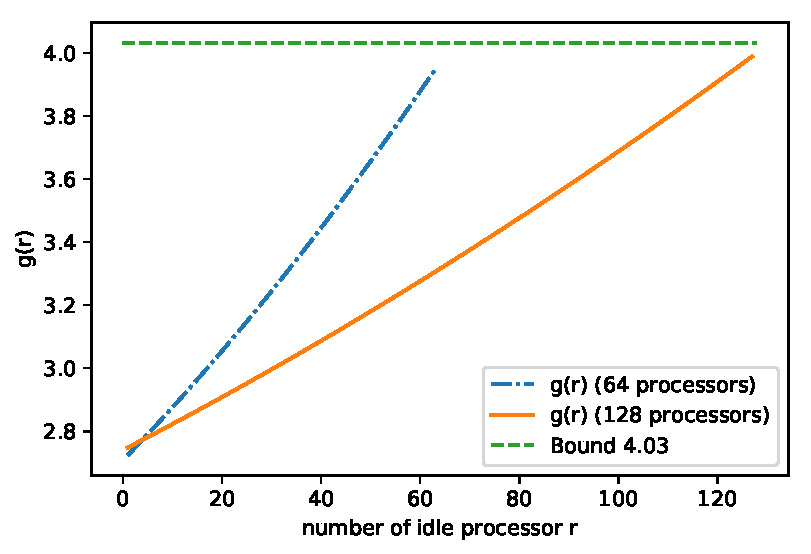
\includegraphics[width=.7\linewidth]{figures/g64}
   \caption{Function $g(r)$ as a function of the number of idle
     processor $r$ for $p=\{64,128\}$ processors. We observe that $g$ is
     increasing and upper bounded by $4.03$. }
   \label{fig:g}
 \end{figure}

 \bigskip

 \subsubsection{Bound $\gamma<4.03$}
 % \begin{lemma}
 % \label{gammabound}
 % \end{lemma}
 % \begin{pf}
   Let define the function $g$ as
   \begin{align}
     \label{eq:g}
     g(r)=\frac{r}{-p\log_2\left(\frac34+\frac14\Big(\frac{p-2}{p-1}\Big)^{r}\right)}.
   \end{align}
   
   By definition, the constant $\gamma$ is the maximum of $g$:
   \begin{align*}
     \gamma=\max_{1\le r \le p-1}g(r).  
   \end{align*}
   
   The function $g$ is displayed in Figure~\ref{fig:g} for the case of
   $64$ processors and $128$ processors. As we observe on this curve,
   $g$ is increasing and is thus bounded by $g(p-1)<4.03$.  This is what we
   prove in the remainder of this proof.

   Let $x=(p-2)/(p-1)$ and $y=x^r$, we have $y\in(0,1)$. We have
   \begin{align*}
     \frac{1}{g(r)} = -p\frac{\log_2(3/4+y/4)}{\log_x(y)} =
     -\frac{p\log x}{\log 2} f(y),
   \end{align*}
   where $f(y)=\log(3/4+y/4)/\log(y)$. The first derivative of $f$ is
   \begin{align*}
     f'(y)=\frac{y\log y - (3+y)\log(3/4+y/4)}{y(3+y)(\log y)^2}.
   \end{align*}
   
   The first derivative of the numerator of $f'(y)$ is
   $\log y - \log (3/4+y/4)$ which is negative for $y<1$. Thus it implies
   that $f'(y)$ is decreasing. As $f'(1)=1$, this shows that
   $f'(y)\ge0$ and therefore that $f$ is increasing. This implies that
   $g(r)$ is increasing (because $y$ is decreasing in $r$ and
   $g(r)=\alpha /f(y)$ for $\alpha=-\log 2 / (p\log x) > 0$).

   As $g$ is increasing, $\gamma = g(p-1)$. Now, for all $ p \geq 2$:
   \begin{align*}
       \left(\frac{p-2}{p-1}\right)^{p-1} & = \left( 1 - \frac{1}{p-1}
     \right)^{p-1}\\
       &= \exp \left((p-1)\ln(1-\frac{1}{p-1}) \right)\\
                     &\leq \exp \left(-(p-1)\frac{1}{p-1} \right) = \frac{1}{e} .
   \end{align*}
   
   This shows that 
      \begin{align*}
     \gamma &= g(p-1) \leq \frac{1}{ 2 - \log_2\left(3 + \frac{1}{e}
              \right)} <  4.03.
   \end{align*}
%  \end{pf}
% \end{pf}

%%% Local Variables:
%%% mode: latex
%%% TeX-master: "main"
%%% End:
